%!tex program = lualatex
\documentclass[answers]{exam}
\usepackage{ctex}
\usepackage{graphicx}
\usepackage[margin=2cm]{geometry}
\usepackage{amsmath, amssymb}
\usepackage{csquotes}
\usepackage{tikz, pgfplots}
\usetikzlibrary{
	angles,
	backgrounds,
	calc,
	decorations.pathmorphing,
	decorations.pathreplacing,
	decorations.text,
	intersections,
	patterns,
	quotes,
	shapes,
	shapes.symbols,
}
\pagestyle{empty}
\newcounter{xcord}
\newcounter{ycord}
\newcounter{total}
\renewcommand{\labelenumi}{\textbf{\ifnum\value{enumi}<10 0\fi\arabic{enumi})}}

\pgfplotsset{compat=1.18}

\CorrectChoiceEmphasis{\color{blue!70!green}\bfseries}
\renewcommand{\solutiontitle}{\textbf{解:}}

\usepackage{array, tabularx}
\newcolumntype{C}{>{\centering\arraybackslash}X}
\newcolumntype{B}{>{\centering\bfseries\arraybackslash}X}
\catcode`\幺=0

\begin{document}
\begin{center}
	\textbf{\large{1977 年普通高等学校招生考试(北京卷) }}

	\textbf{\LARGE{理科数学}}
\end{center}
\begin{questions}
	\question 解方程: \( \sqrt{x - 1} = 3 - x \).
	\begin{solution}
		\begin{align*}
			\sqrt{x - 1}  & = 3 - x        \\
			x - 1         & = 9 - 6x + x^2 \\
			x^2 - 7x + 10 & = 0            \\
			(x-2)(x-5)    & = 0            \\
			x_1 = 2, x_2 = 5
		\end{align*}
	\end{solution}

	\question 计算: \( 2^{-\frac12} + \frac{2^0}{\sqrt{2}} + \frac{1}{\sqrt{2} - 1}. \)

	\begin{solution}
		\begin{align*}
			\text{原式} & = \frac{1}{\sqrt{2}} + \frac{1}{\sqrt{2}} + \sqrt{2} + 1 \\
			          & = \frac{2}{\sqrt{2}} + \sqrt{2} + 1                      \\
			          & = 2\sqrt{2} + 1
		\end{align*}
	\end{solution}

	\question 已知 \( \lg2 = 0.3010, \lg3 = 0.4771, \) 求 \( \lg\sqrt{45} \).

	\begin{solution}
		\begin{align*}
			\lg\sqrt{45} & = \frac12\lg{45}                        \\
			             & = \frac12(\lg5 + \lg9)                  \\
			             & = \frac12(\lg5 + 2\lg3)                 \\
			             & = \frac12(\lg\frac{10}{2} + 2\lg3)      \\
			             & = \frac12(\lg10 - \lg2 + 2\lg3)         \\
			             & = \frac12(1 - 0.3010 + 2 \times 0.4771) \\
			             & = 0.8266
		\end{align*}
	\end{solution}

	\question 证明: \( (1 + \tan\alpha)^2 = \dfrac{1 + \sin2\alpha}{\cos^2\alpha} \)。
	\begin{solution}
		\begin{align*}
			(1+\tan\alpha)^2
			           & = \left(1 + \frac{\sin\alpha}{\cos\alpha}\right)^2  \text{(将 \(\tan\alpha = \frac{\sin\alpha}{\cos\alpha}\) 代入)} \\
			           & = \left(\frac{\cos\alpha + \sin\alpha}{\cos\alpha}\right)^2 \text{(通分并化简分母)}                                     \\
			           & = \frac{(\cos\alpha + \sin\alpha)^2}{\cos^2\alpha}                                                               \\
			           & = \frac{\cos^2\alpha + 2\cos\alpha\sin\alpha + \sin^2\alpha}{\cos^2\alpha}                                       \\
			           & = \frac{1 + 2\cos\alpha\sin\alpha}{\cos^2\alpha}                                                                 \\
			           & \text{(根据三角恒等式 \(\cos^2\alpha + \sin^2\alpha = 1\) 化简)}                                                          \\
			           & = \frac{1 + \sin2\alpha}{\cos^2\alpha}                                                                           \\
			           & \text{(利用 \(\sin2\alpha = 2\cos\alpha\sin\alpha\))}                                                              \\
			\therefore & \, (1+\tan\alpha)^2 = \frac{1 + \sin2\alpha}{\cos^2\alpha}。
		\end{align*}
	\end{solution}

	\question 求过两直线 \( x + y - 7 = 0 \) 和 \( 3x - y - 1 = 0 \) 的交点且过 \( (1, 1) \) 点的直线方程。
	\begin{solution}
		\begin{align*}
			 & \begin{cases}
				   x + y - 7 = 0, \\
				   3x - y - 1 = 0
			   \end{cases}                                                                \\
			 & \text{解得:} x = 2, \, y = 5,\text{即交点为 } (2, 5)。                               \\
			 & \text{过点 } (2,5) \text{ 和 } (1,1) \text{ 的直线斜率:} k = \frac{5 - 1}{2 - 1} = 4。 \\
			 & \text{设直线方程为:} y = 4x + a,\text{将 } (1,1) \text{ 代入,得:}                       \\
			 & a = -3。                                                                       \\
			 & \text{因此,所求直线方程为:} y = 4x - 3。
		\end{align*}
	\end{solution}

	\question 某工厂今年七月份的产值为 \( 100 \)万元,以后每月产值比上月增加 \( 20\%
	\),问今年七月份到十月份总产值是多少?

	\begin{solution}
		\begin{align*}
			\text{根据等比数列求和公式} S_n = a_1\frac{1- q^n}{1-q}                    \\
			\text{代入}  a_1 = 100, q = 1.2, n = 4  \text{得:}                  \\
			S_4 & = 100 \times \frac{1 - 1.2^4}{1 - 1.2}                     \\
			    & = 100 \times \frac{(1 - 1.2)(1 + 1.2)(1 + 1.2^2)}{1 - 1.2} \\
			    & = 100 \times 2.2 \times 2.44                               \\
			    & = 536.8 \text{(万元)}
		\end{align*}

	\end{solution}

	\question 已知二次函数 \( y = x^2 - 6x + 5 \)
	\begin{enumerate}[label=(\arabic*)]
		\item 求出它的图像的顶点坐标和对称轴方程;
		\item 画出它的图像;
		\item 分别求出它的图像和 \( x \)轴、$ y $的交点坐标.
	\end{enumerate}

	\begin{solution}
		\begin{enumerate}[label=(\arabic*)]
			\item
			      \begin{align*}
				      \text{对称轴的方程为} x = -\frac{b}{2a} & = 3,  \\
				      \text{将} x = 3 \text{代入得:} y     & = -4, \\
			      \end{align*}
			\item
			      \begin{center}
				      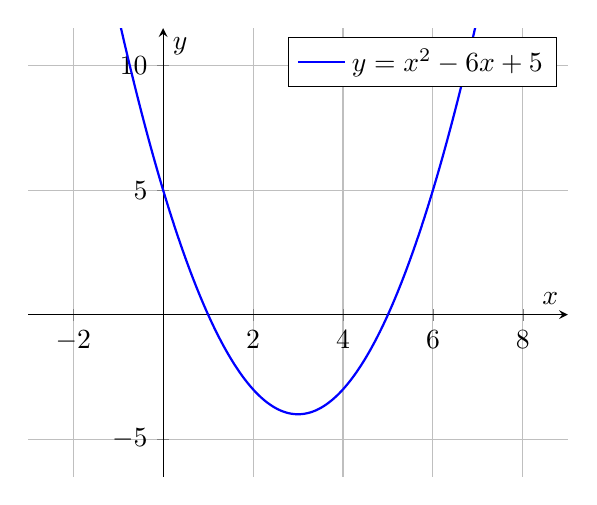
\begin{tikzpicture}
					      \begin{axis}[
							      axis lines=middle,          % 坐标轴通过原点
							      xlabel={$x$}, ylabel={$y$}, % 坐标轴标签
							      grid=major,                 % 显示网格
							      xmin=-2, xmax=8,            % x轴范围
							      ymin=-5, ymax=10,           % y轴范围
							      domain=-4:8,                % 定义函数绘制范围
							      samples=100,                % 样本点数,越大曲线越平滑
							      enlargelimits=true,         % 扩展范围
						      ]
						      % 绘制抛物线 y = ax^2 + bx + c
						      \addplot[smooth, thick, blue] {x^2 - 6*x + 5};
						      % 添加图例
						      \addlegendentry{$y = x^2 - 6x + 5$}
					      \end{axis}
				      \end{tikzpicture}
			      \end{center}

			\item \begin{align*}
				      y & = x^2 - 6x + 5                            \\
				        & = (x - 1)(x - 5)                          \\
				        & \text{则有两个交点分别为:} (1, 0) \text{和} (5, 0).
			      \end{align*}
		\end{enumerate}

	\end{solution}

	\question 一只船以 $20$ 海里/小时的速度向正东航行, 起初船在 $A$处看见一灯塔 $B$ 在船的北 $45^\circ$ 东方向, 一小时后船在
	$C$ 处看见这个灯塔在船的北 $15^\circ$ 东方向, 求这时船和灯塔的距离 $CB$.

	\begin{solution}\\
		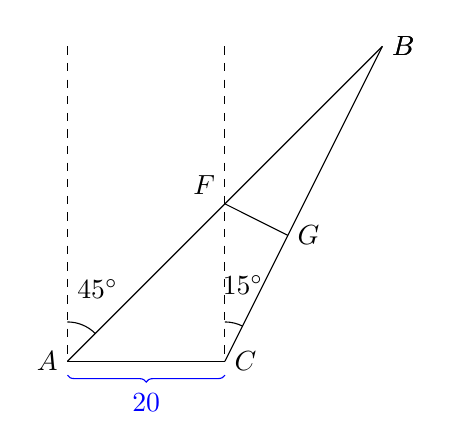
\begin{tikzpicture}
			\coordinate(A) at (0,0);
			\coordinate(B) at (4,4);
			\coordinate(C) at (2,0);
			\coordinate(D) at (0,4);
			\coordinate(E) at (2,4);
			\draw[dashed] (D)  -- (A)node[left]{$A$};
			\draw[name path=AB] (A) --  (B)node[right]{$B$};
			\pic["$45^\circ$", draw, angle eccentricity=2] {angle=B--A--D};
			\draw (A) -- (C)node[right] {$C$};
			\draw[decorate, decoration={brace, mirror, raise=5pt}, blue, draw] (A) --node[midway, below=8pt]{20} (C);
			\draw (C)-- (B)node[right]{$B$};
			\draw[dashed, name path=CE] (E) -- (C);
			\pic["$15^\circ$", draw, angle eccentricity=2] {angle=B--C--E};
			\path [name intersections={of=AB and CE, by=F}];
			\node[above left] at (F) {$F$};
			\coordinate(G) at ($(C)!(F)!(B)$);
			\draw (F) -- (G)node[right]{$G$};
		\end{tikzpicture}
		\begin{tikzpicture}
			\tkzDefPoint(0,0){A}  % 定义点 A
			\tkzDefPoint(4,4){B}  % 定义点 B
			\tkzDefPoint(2,0){C}  % 定义点 C
			\tkzDefPoint(0,4){D}  % 定义点 D
			\tkzDefPoint(2,4){E}  % 定义点 E

			% 绘制点
			\tkzDrawPoints(A,B,C,D,E)

			% 绘制线段
			\tkzDrawSegments(A,B B,C C,D)
			\tkzDrawSegment[draw,dashed](A,D)  % 虚线
			\tkzDrawSegment[draw,dashed](C,E)  % 虚线

			% 标记角度
			\tkzMarkAngle[draw=blue,fill=blue,angle radius=1cm](B,A,D)
			\tkzLabelAngle[sloped, pos=1.5](B,A,D){$45^\circ$}
			\tkzMarkAngle[draw=red,fill=red,angle radius=1cm](B,C,E)
			\tkzLabelAngle[sloped, pos=1.5](B,C,E){$15^\circ$}

			% 在某些点上标记标签
			\tkzLabelPoint[below left](A){$A$}
			\tkzLabelPoint[above right](B){$B$}
			\tkzLabelPoint[below](C){$C$}
			\tkzLabelPoint[above](D){$D$}
			\tkzLabelPoint[above](E){$E$}

			% 绘制带有标签的标注
			\tkzDrawSegment(A,C)
			\tkzLabelSegment[below](A,C){20}

			% 寻找交点 F,并绘制直线
			\tkzInterLL(A,B)(C,E) \tkzGetPoint{F}
			\tkzDrawPoints(F)
			\tkzLabelPoint[above left](F){$F$}

			% 绘制直线 FG
			\tkzDefPointBy[projection=onto B--C](F) \tkzGetPoint{G}
			\tkzDrawSegment(F,G)
			\tkzLabelPoint[right](G){$G$}
		\end{tikzpicture}

		\begin{itemize}
			\item \textbf{确定三角形} $\triangle{ACF}$ 是等腰直角三角形,得出:
			      \[
				      CF = AC = 20 \text{(海里)}.
			      \]
			\item \textbf{角度关系}:设 $\alpha = 15^\circ$,则:
			      \[
				      FG = \sin{\alpha} \cdot FC, \quad CG = \cos{\alpha} \cdot FC.
			      \]
			\item \textbf{角度推导}:由三角形角度关系得:
			      \[
				      \angle ABC = 180^\circ - \angle CAB - 90^\circ - 15^\circ = 30^\circ.
			      \]
			\item \textbf{计算 BG}:使用三角关系得:
			      \[
				      BG = \sqrt{3} \cdot FG.
			      \]
			\item \textbf{求解BC}: 综合前述公式得:
			      \[
				      BC = BG + CG = \sqrt{3} \cdot 20 \cdot \sin{\alpha} + 20 \cdot \cos{\alpha}.
			      \]
			\item \textbf{最终结果}:
			      \[
				      BC^2 = 400 \left( 3 \sin^2{\alpha} + 2\sqrt{3} \sin{\alpha} \cos{\alpha} + \cos^2{\alpha} \right).
			      \]
			\item \textbf{化简倍角公式}:
			      \[
				      \text{倍角公式:} \sin{2\alpha} = 2 \sin{\alpha} \cos{\alpha}, \quad \sin^2{\alpha} + \cos^2{\alpha} = 1,
			      \]
			      得到:
			      \[
				      BC^2 = 400 \left( 2 \sin^2{\alpha} + \sqrt{3} \sin{2\alpha} + 1 \right).
			      \]
			\item \textbf{最后化简}:
			      \[
				      BC^2 = 400 \left( 1 - \frac{\sqrt{3}}{2} + \frac{\sqrt{3}}{2} + 1 \right),
			      \]
			      最终得出:
			      \[
				      BC = 20\sqrt{2} \text{(海里)}.
			      \]
		\end{itemize}
	\end{solution}

	\question 一个圆内接三角形 \( ABC \),$\angle A$的平分线交$BC$于$D$,交外接圆于$E$,求证: \( AD \cdot AE = AC \cdot
	AB\).

	\begin{solution}
		\begin{minipage}{.4\textwidth}
			\begin{tikzpicture}
				\tkzDefPoint (0,0){A}
				\tkzDefPoint (5,0){B}
				\tkzDefPoint (3,4){C}

				% 外接圆
				\tkzCircumCenter(A,B,C) \tkzGetPoint{O}
				\tkzDrawCircle(O,A)

				% 角平分线
				\tkzDefLine[bisector](B,A,C) \tkzGetPoint{a}
				\tkzInterLL(A,a)(B,C) \tkzGetPoint{D}
				\tkzInterLC(A,a)(O,A) \tkzGetPoints{A}{E}
				\tkzDrawSegment(A,E)

				\tkzDrawPolygon(A,B,C)
				\tkzLabelPoints(A,B)
				\tkzLabelPoint[above](C){$C$}
				\tkzLabelPoint[above left](D){$D$}
				\tkzLabelPoint[right](E){$E$}
			\end{tikzpicture}
		\end{minipage}

	\end{solution}

\end{questions}

\end{document}
